\documentclass[11pt,a4paper]{article}
\usepackage[english]{babel}
\usepackage[utf8]{inputenc}
\usepackage{amsmath}
\usepackage{graphicx}
\usepackage{caption}
\usepackage{float}
%\usepackage[margin=1.25in]{geometry}
\usepackage[numbered,framed]{matlab-prettifier}
\usepackage{filecontents}
\usepackage[T1]{fontenc}
\usepackage{bigfoot}
\usepackage{listings}

\numberwithin{equation}{subsection}


\begin{filecontents*}{h1.m}
	 % Load the data
	 clear all; close all; clc;
	 load Testdata
	 
	 L = 15; % spatial domain
	 n = 64; % Fourier modes
	 x2 = linspace(-L, L, n + 1); x = x2(1: n);  y = x;  z = x;
	 k = (2 * pi / (2 * L)) * [0: (n / 2 - 1) -n / 2: -1];  ks = fftshift(k);
	 
	 [X, Y, Z] = meshgrid(x, y, z);
	 [Kx, Ky, Kz] = meshgrid(ks, ks, ks);
	 
	 % Plot the Original data at 20th measurement
	 figure(1)
	 Un_init(:, :, :) = reshape(Undata(20, :), n, n, n);
	 isosurface(X ,Y , Z, abs(Un_init), 0.4)
	 axis([-20 20 -20 20 -20 20]), grid on, pbaspect([1 1 1])
	 set(gca, 'Fontsize', [12])
	 xlabel('space(x)'); ylabel('space(y)');zlabel('space(z)');
	 
	 % Unfiltered FFT
	 Untave=0;
	 for j = 1: 20
	     Un(:, :, :) = reshape(Undata(j, :), n, n, n);
	     Unt = fft(fft(fft(Un, [], 1), [], 2), [], 3);
	     Untave = Untave + Unt;
	 end
	 Untave=fftshift(Untave)/20;
	 Untp = abs(Untave) / max(abs(Untave(:)));
	 
	 % Find the coordinates for the frequency signature and plot it
	 [cx, cy, cz] = ind2sub(size(Untave), find(abs(Untave) == max(abs(Untave(:)))));
	 figure(2)
	 isosurface(Kx, Ky, Kz, Untp, 0.6)
	 axis([-2*pi 2*pi  -2*pi 2*pi  -2*pi 2*pi]), grid on, pbaspect([1 1 1])
	 set(gca, 'Fontsize', [12])
	 xlabel('frequency(Kx)'); ylabel('frequency(Ky)');zlabel('frequency(Kz)');
	 
	 % Create the Gaussian filter of the form exp(-0.2*(k - k0) .^ 2)
	 K0 = [Kx(cx, cy, cz), Ky(cx, cy, cz), Kz(cx, cy, cz)];
	 cent_freq = K0*(2 * L / (2 * pi));
	 filter = exp(-0.2*((Kx - K0(1)) .^ 2 + (Ky - K0(2)) .^ 2 +  (Kz - K0(3)) .^ 2));
	 
	 % Apply FFT with the Gaussian filter
	 figure(3)
	 pos = zeros(20, 3);
	 for j = 1:20
	     Un(:, :, :) = reshape(Undata(j, :), n, n, n);
	     Unt = fft(fft(fft(Un, [], 1), [], 2), [], 3);
	%      Unt = fftn(Un);
	     Untf = filter .* fftshift(Unt);
	     Unf = ifft(ifft(ifft(Untf, [], 1), [], 2), [], 3);
	     Unfp = abs(Unf)/ max(abs(Unf(:)));
	 
	     % Plot the marble for each measurement on isosurface
	     subplot(1, 2, 1)
	     isosurface(X, Y, Z, Unfp, 0.8)
	     axis([-20 20 -20 20 -20 20]), grid on, pbaspect([1 1 1]), drawnow
	     set(gca, 'Fontsize', [12])
	     xlabel('space(x)'); ylabel('space(y)');zlabel('space(z)');
	     pause(0.1)
	 
	     % Find the exact coordinates of the marble of each measurement in
	     % spatial domain
	     [cx, cy, cz] = ind2sub(size(Unf), find(abs(Unf) == max(abs(Unf(:)))));
	     pos(j, :) = [X(cx, cy, cz), Y(cx, cy, cz), Z(cx, cy, cz)];
	 end
 
 % Plot the trajectory of the marble
 subplot(1, 2, 2)
 plot3(pos(:, 1), pos(:, 2), pos(:, 3), 'ro-', 'Linewidth', [2])
 axis([-20 20 -20 20 -20 20]), grid on, pbaspect([1 1 1])
 set(gca, 'Fontsize', [12])
 xlabel('space(x)'); ylabel('space(y)');zlabel('space(z)');
 final_pos = pos(20, :);

\end{filecontents*}
\let\ph\mlplaceholder % shorter macro
\lstMakeShortInline"

\lstset{
  style              = Matlab-editor,
  basicstyle         = \mlttfamily,
  escapechar         = ",
  mlshowsectionrules = true,
}

\title{Amath 482 Winter 2019 \\
HW1: An ultrasound problem}

\author{Wenrui Yuan}

\date{\today}

\begin{document}

\maketitle


\begin{abstract}
This report performs a frequency analysis on a dataset. The data includes twenty ultrasound measurements of a marble in a dog's intestine, which is hard to identify due to internal fluids and the dog's movement. The approach is to perform a fast Fourier Transform and spectrum averaging to compute frequency signature of the marble, which will be used to study the trajectory of it and determine the final position where should an acoustic wave be focused to disintegrate it.
\end{abstract}


\section{Introduction and Overview}
\label{sec:introduction}
The original data in this problem from ultrasound detection of the intestine is full of noise (as shown in later figures) and thus considered relatively useless. Moreover,  movement of internal fluids make it extremely hard to locate the marble.
\\Therefore, using the FFT algorithm to decompose the data into frequency components is necessary. We must locate the marble by averaging the spectrum to compute the central frequency. The we create a proper Gaussian filter to the signal around the frequency to obtain coordinated of the marble at each measurement. As soon as the position at the final measurement is located, an intense acoustic wave can be applied to break up the marble. Techniques and algorithm used in this frequency analysis will be covered in following sections.



\section{Theoretical Background}
\label{sec:theory}

	\subsection{Fourier Transform}
	The idea of frequency analysis is to decompose the function of time(space) into its frequency components. One major approach is to apply the Fourier Transform, defined over the entire line $x \in [-\infty, \infty]$ as \cite{582notes}
		\begin{equation}
		\hat{f}(k)=\frac{1}{\sqrt{2\pi}}\int_{-\infty}^{\infty} f(x)e^{-ikx}dx
		\end{equation}
		whereas the inverse is defined as \cite{582notes}
		\begin{equation}
		f(x)=\frac{1}{\sqrt{2\pi}}\int_{-\infty}^{\infty}\hat{f}(x)e^{ikx}dk
		\end{equation}
	However, as we are only interested in over a finite domain $x \in [-L, L]$, the transform(a continuous eigenfunction expansion) is simply the direct sum of eigenfunctions and associated wavenumber $k$.\cite{582notes}
	
	\subsection{FFT: Fast Fourier Transform}
	In order to perform the Fourier transform for frequency analysis on a dataset of size \texttt{20x262144}, we use the FFT algorithm due to its high accuracy and low time complexity $\mathcal{O}(N log N)$. However, it divides and conquers the Fourier transform into smaller ones\cite{fft_wiki} and thus requires the finite domains to be discretized into $2^N$ points.\cite{582notes}
	
	\subsection{Spectrum Averaging}
	Spectrum averaging is very powerful in eliminating white noises as they can be defined as a normally distributed random variable with zero mean\cite{582notes}. This helps us to identify frequency signature(central frequency) of the object that we are interested in. Once the frequency signature is acquired, we may build a Gaussian filter to further denoise the data.
	
	\subsection{Gaussian Filter}
	As mentioned in the averaging method, we will need the central frequency to build the filter as a Gaussian filter is normally defined as \cite{582notes}:
		\begin{equation}
		\mathcal{F}(x) = \exp (-\tau (k-k_0)^2)
		\end{equation}
	In particular, this filter isolates the frequency around $k_0$ and attenuates all other frequencies.


\section{Algorithm Implementation and Development}
	\begin{enumerate}
		\item \textbf{Load \texttt{testdata.mat}}
		
		\item \textbf{Set wavenumber $k$}\\ 
		We will need frequency components of FFT as the algorithm assumes the $2\pi$ period. Moreover, it must be shifted back to its mathematically correct position via the \texttt{fftshift} function as FFT will results in shifts of the domain that $[-L, 0] \rightarrow [0, -L]$ and $[0, L] \rightarrow [L, 0]$.\cite{582notes}
		
		\item \textbf{Create spatial and frequency grids in 3D using \texttt{meshgrid}}
		
		\item \textbf{Reshape data at each measurement into a 3-D matrix using \texttt{reshape}}
		
		\item \textbf{For each measurement, \texttt{fft} reshaped data on every dimensions}
		\item \textbf{Use a variable \texttt{Untave} to sum transformed data and \texttt{fftshift} it}. 
		\\ Divide \texttt{Untave} by the number of measurements(20) to get spectrum average.
		
		\item \textbf{Find coordinate of central frequency using \texttt{ind2sub}}
		\\ Find central wavenumber $k_0 = [K_x, K_y, K_z]$ using the coordinate. Multiply $k_0$ by $2(\frac{L}{2\pi})$ to to get the central frequency.
		
		\item \textbf{Visualize \texttt{Untave} on \texttt{isosurface} by normalizing it with its maximum element}
		
		\item \textbf{Create a 3-D Gaussian filter around $k_0$}
		
		\item \textbf{Apply \texttt{reshape} and \texttt{fft} again to the data at each measurement}
		
		\item \textbf{Multiply each transformed data with filter and inverse transform it using \texttt{ifft}}
		
		\item \textbf{\texttt{fftshift} the filtered signal and normalize it with its maximum}
		
		\item \textbf{Visualize the marble for each measurement on \texttt{isosurface}}
		
		\item \textbf{Compute coordinates in space domain of the marble at all measurements}
		\\ Method used here is identical as in step 7. We take the $xyz$ indices of strongest signals at each measurement into predefined spatial grid $[X, Y, Z]$ to compute the set of coordinates in space domain.
		
		\item \textbf{Plot trajectory of the marble}
	\end{enumerate}


\section{Computational Results}
We start with the noisy data as shown in the figure 1(\texttt{isovalue=0.4}). There's no clear sign of the marble anywhere in the domain.\\

	\begin{figure}[H]
		\begin{center}
			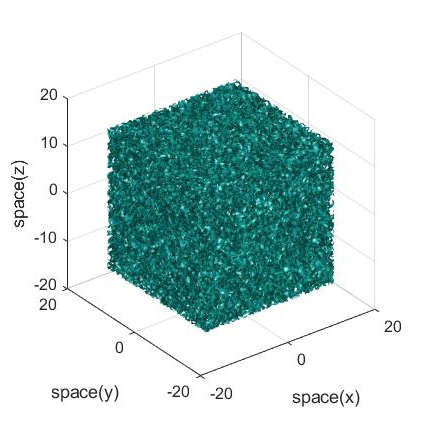
\includegraphics[scale=0.60]{Figure1.jpg}
			\caption{Isosurface visualization for the 20th measurement in space domain}
		\end{center}
	\end{figure}

After the initial FFT and spectrum averaging, the marble is recognizable as shown in figure 2(\texttt{isovalue=0.6}), which implicates the frequency signature $k_0 = [1.8850, -1.0472, 0]$ of the marble with only a few noises. We then find its central frequency at $[9, -5, 0]$ (factor $k_0$ by $\frac{2L}{2\pi}$, as the $L$ presents in code is in fact $\frac{L}{2}$).\\

	\begin{figure}[H]
		\begin{center}
			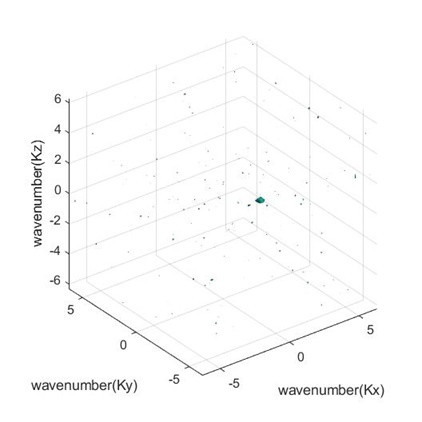
\includegraphics[scale=0.60]{Figure2.jpg}
			\caption{Isosurface visualization after spectrum averaging}
		\end{center}
	\end{figure}

By creating the Gaussian filter with $k_0$, visualization of the isosurface at all time(\texttt{isovalue=0.8}) and trajectory of the marble are shown in figure 3.

	\begin{figure}[H]
		\begin{center}
			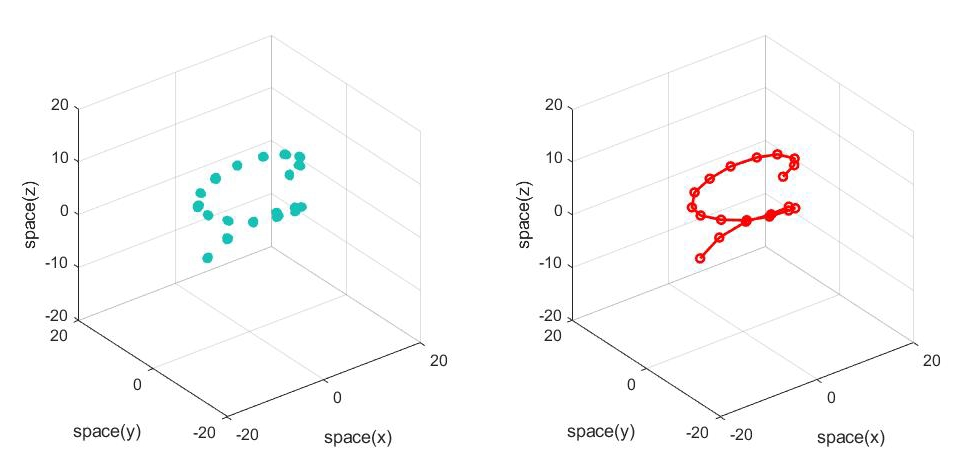
\includegraphics[scale=0.50]{Figure3.jpg}
			\caption{Isosurface visualization of the marble at all 20 measurements in space(left) and the trajectory of the marble(right)}
		\end{center}
	\end{figure}


\section{Summary and Conclusions}
The main idea of this analysis is to denoise the 3D data in space domain through Gaussian filtering. We constructed such filter by averaging spectrum and are thus able to locate frequency signature of the marble. Once we have the filtered signal by filtering transformed data, the position of the marble at the 20th time measurement is on $[-5.6250, 4.2188, -6.0938]$, where an intense acoustic wave should be focused to break up the marble.


\begin{thebibliography}{11}
	\bibitem{582notes}
	J. Nathan Kutz. 2013.
	\textit{Data-Driven Modeling \& Scientific Computation}. p. 27-48
	
	\bibitem{fft_wiki}
	\textit{Cooley-Tukey FFT algorithm. Wikipedia}; [2019 Jan 23]. \\https://en.wikipedia.org/wiki/Cooley\- Tukey\_ FFT\_ algorithm
\end{thebibliography}

\pagebreak
\section*{Appendix A: MATLAB functions used}
	\begin{itemize}
		\item \lstinline{meshgrid}\\ Creates 2-D or 3-D grid with specified vectors.
		\item \lstinline{isosurface}\\ Visualizes the isosurface with specified isovalues.
		\item \lstinline{reshape}\\Reshapes the array or matrix into specific shape.
		\item \lstinline{fft}\\Performs the Fourier Transform via FFT algorithm. In particular, \lstinline{fft(Un,[],n)}is used to perform the transform in n-th dimension.
		\item \lstinline{fftshift}\\ Shift the zero-frequency to center of the spectrum.
		\item \lstinline{ifft}\\ Performs the inverse Fourier transform.
		\item \lstinline{ind2sub}\\ Returns an array subscripts of given indices with specified size.
		\item \lstinline{find}\\ Returns the index(indices) of specified elements.
		\item \lstinline{plot3}\\ Plot 3-D lines with given points of data.
	\end{itemize}

\section*{Appendix B: MATLAB codes}
\lstinputlisting{h1.m}

\end{document}